\part{Profiler}
\frame{\partpage}

\begin{frame}{UE4}
	\begin{center}
		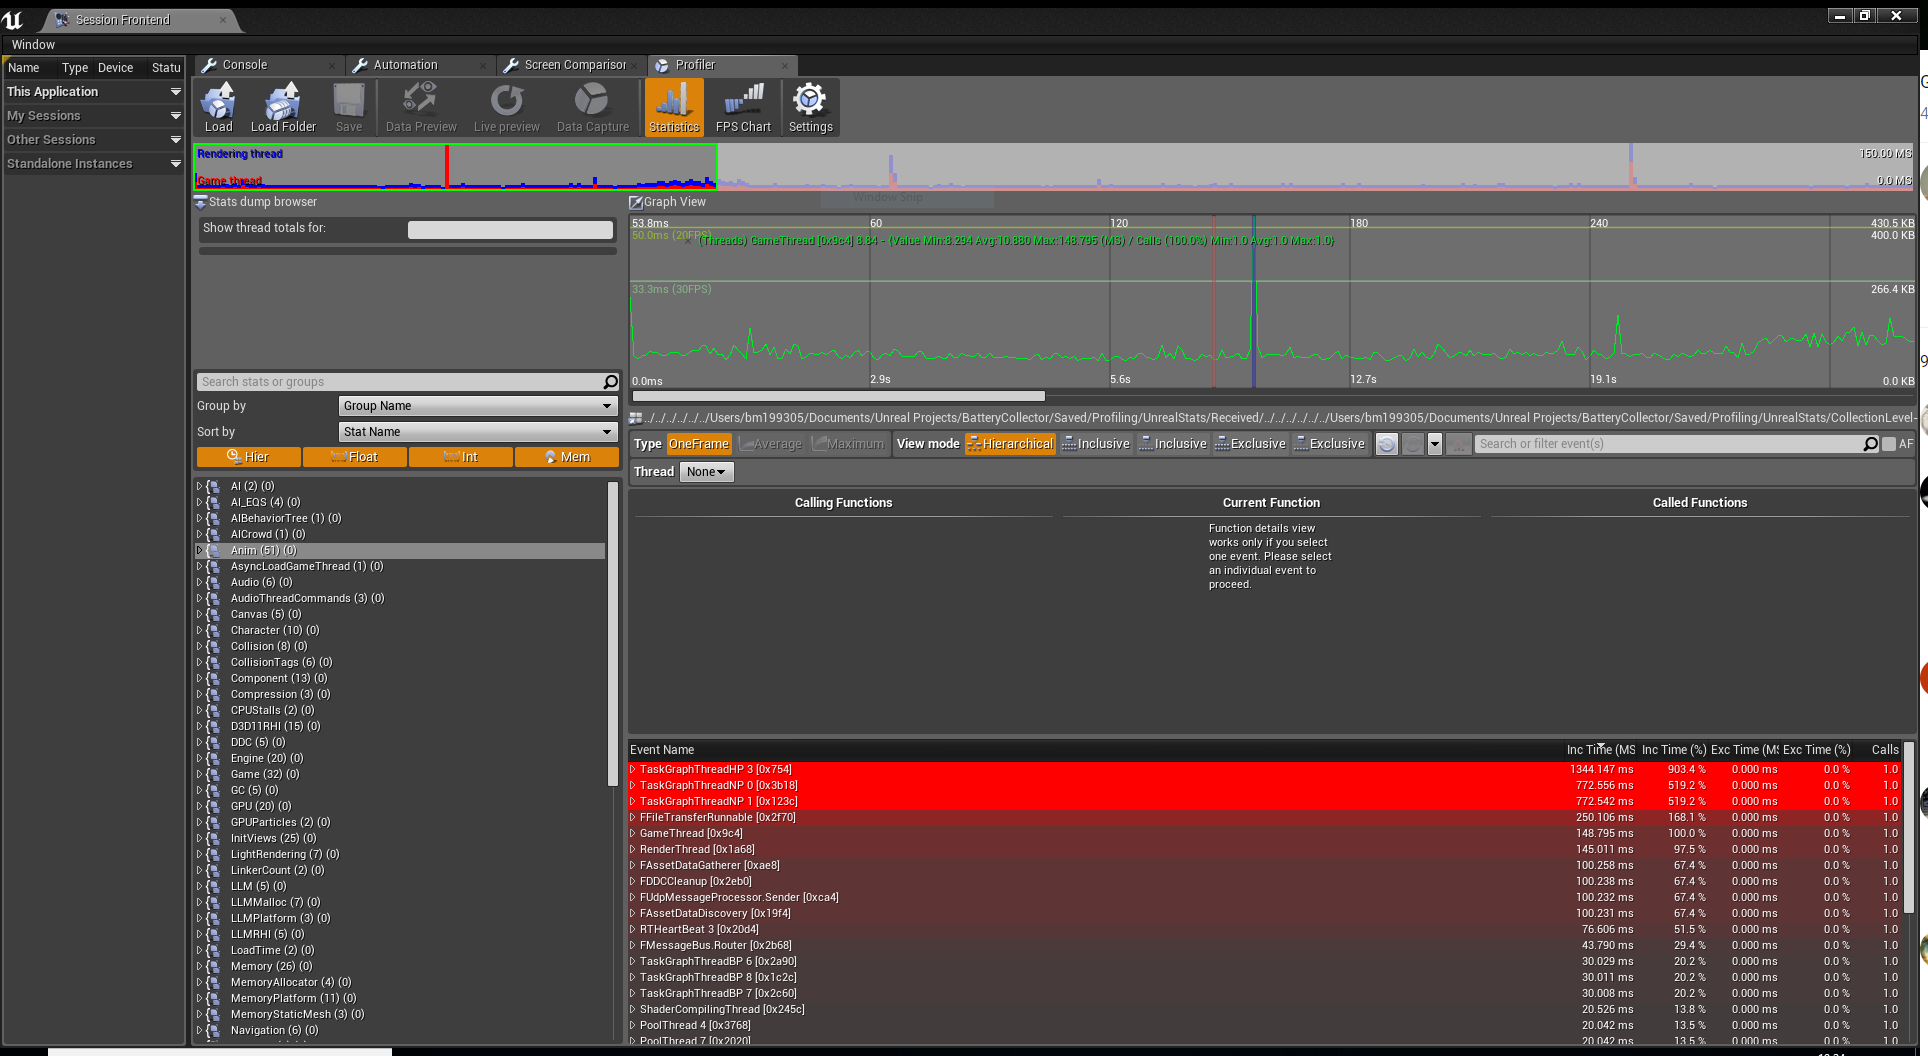
\includegraphics[width=\textwidth,height=\textheight,keepaspectratio]{UnrealProfilerWindow}
	\end{center}
\end{frame}


\begin{frame}{Unity}
	\begin{center}
		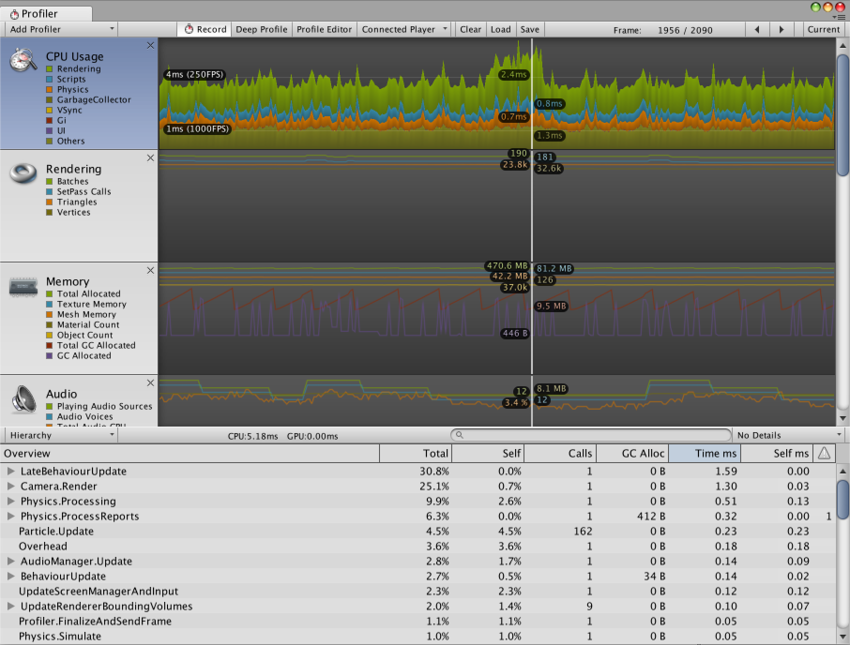
\includegraphics[width=\textwidth,height=\textheight,keepaspectratio]{UnityProfilerWindow}
	\end{center}
\end{frame}

\begin{frame}{Profiler}
	\begin{itemize}
		\item You have already met the profilers for UE4 and Unity
		\item They have some commonalities
		\begin{itemize}
			\item Visualise Performance via graphs
			\item Performance measures (calls, time, frame time etc)
			\item Code call graphs, usually linked to the visuals and perf measures
		\end{itemize}
		\item This is the main tool you have to measure performance in your game
	\end{itemize}
\end{frame}

\begin{frame}{Profiling Tips}
	\begin{itemize}
		\item Run the profiler on a built version of your game
		\item Turn off features of the profiler you don't need
	\end{itemize}
\end{frame}